\documentclass{standalone}
\usepackage{tikz}
\usepackage{ctex,siunitx}
\usepackage{tkz-euclide}
\usepackage{amsmath}
\usetikzlibrary{patterns, calc}
\usetikzlibrary {decorations.pathmorphing, decorations.pathreplacing, decorations.shapes,}
\begin{document}
\small
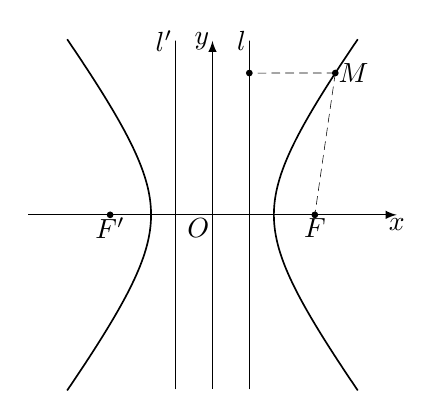
\begin{tikzpicture}[>=latex,scale=1.3,inner sep=1pt]
  \draw[thin,->](-1.8,0)--(1.8,0)node[below]{$x$};
  \draw[thin,->](0,-1.7)--(0,1.7)node[left]{$y$};
  \tkzDefPoints{0/0/O,-1/0/F1,1/0/F2,0.36/1.7/A,0.36/-1.7/B,-0.36/-1.7/C,-0.36/1.7/D}
  \draw[semithick,domain=-65:65,samples=200] plot ({0.6/cos(\x)},{0.8*tan(\x)});
  \draw[semithick,domain=-65:65,samples=200] plot ({-0.6/cos(\x)},{0.8*tan(\x)});
  \tkzDefPoint(1.2,{0.8*sqrt(3)}){M}
  \tkzDefPointBy[projection=onto A--B](M)\tkzGetPoint{Q}
  \tkzDrawSegments[densely dashed](M,Q M,F2)
  \tkzDrawPoints[fill=black](M,F1,F2,Q)
  \tkzLabelPoints[right](M)
  \tkzLabelPoint[below](F1){$F'$}
  \tkzLabelPoint[below](F2){$F$}
  \tkzDrawLine[add=0 and 0](A,B)
  \tkzLabelLine[pos=0,left](A,B){$l$}
  \tkzDrawLine[add=0 and 0](C,D)
  \tkzLabelLine[pos=1,left](C,D){$l'$}
  \tkzLabelPoints[below left](O)
  % \node at (0,0.8)[above right]{$B_2$};
  % \node at (0,-0.8)[below right]{$B_1$};
  % \node at (-0.6,0)[above right]{$A_1$};
  % \node at (0.6,0)[above left]{$A_2$};
  % \node at (0.3,0)[below]{$a$};
  % \node at (0,0.4)[left]{$b$};
\end{tikzpicture}
\end{document}